
%%
%% OSDI 2014 Submission requirements
%% 12 pages + plus as many pages as needed for references.
%%
%% Blind reviewing of full papers will be done by the program committee
%% and external review committee, with limited use of outside
%% referees. Authors must make a good faith effort to anonymize their
%% submissions, and they should not identify themselves either explicitly
%% or by implication (e.g., through the references or
%% acknowledgments). Submissions violating the detailed formatting and
%% anonymization rules will not be considered for publication.

% Usenix/OSDI requirements 
\documentclass[10pt,twocolumn]{article}
\usepackage{times}
\usepackage{fullpage}

% added for our purpose
%\usepackage{authblk}
\usepackage{xspace}
\usepackage{url}
\usepackage{upgreek}
\usepackage{comment}
\usepackage{graphicx}
\usepackage{subfig}
\usepackage[normalem]{ulem}
\usepackage[hidelinks]{hyperref}
% name of the product in a funky font
\newcommand{\microsecond}{$\upmu{}$s\xspace}
\newcommand{\ix}{\textsc{ix}\xspace}
\newcommand{\twiddle}{$\sim$}

%%%%%%%%%%%%%%%%%%%%%%%%%%%%%%%%%
% SQUEEZING SPACE

\usepackage[compact]{titlesec}%squeeze

%\newcommand{\myparagraph}[1]{{\bf #1}}
%\newcommand{\myparagraph}[1]{\paragraph{#1}}
%\newcommand{\myparagraph}[1]{{\vspace{5pt}\noindent\bf #1}}
\newcommand{\myparagraph}[1]{{\vspace{3pt}\noindent\bf #1}}

%\addtolength{\parskip}{-5pt}
\addtolength{\abovecaptionskip}{-5pt}
\addtolength{\belowcaptionskip}{-10pt}

%%%%%%%%%%%%%%%%%%%%%%%%%%%%%%%%
% debugging only
\usepackage[usenames,dvipsnames]{xcolor}
\newif\ifcomments
\commentstrue

%% Uncomment the following line to remove comments from text and get an
%% accurate page count.
\commentsfalse

\ifcomments
\newcommand{\edb}[1]{\noindent{\color{Plum} {\bf \fbox{EdB} {\it#1}}}}
\newcommand{\adam}[1]{\noindent{\color{Red} {\bf \fbox{AB} {\it#1}}}}
\newcommand{\christos}[1]{\noindent{\color{Green} {\bf \fbox{CK} {\it#1}}}}
\newcommand{\george}[1]{\noindent{\color{Blue} {\bf \fbox{GP} {\it#1}}}}
\newcommand{\ana}[1]{\noindent{\color{Orange} {\bf \fbox{AK} {\it#1}}}}
%\newcommand{\babak}[1]{\noindent{\color{Purple} {\bf \fbox{BF}} {\it#1}}}
\newcommand{\dm}[1]{\noindent{\color{Red}{\fbox{DM} {#1}}}}
\newcommand{\todo}{\noindent $\triangleright $~}
\else
\newcommand{\edb}[1]{}
\newcommand{\adam}[1]{}
\newcommand{\christos}[1]{}
\newcommand{\george}[1]{}
\newcommand{\ana}[1]{}
\newcommand{\dm}[1]{}
\newcommand{\todo}[1]{}
\fi
\newcommand{\oldcite}[2]{\item #1 ({\small #2})\cite{#2}.}

%%%%%%%%%%%%%%%%%%%%%%%%%%%%%%%%%%%%%%%%%%%%
\begin{document}

%%%%%% TITLE OPTIONS
%\title{\bf Title}
%\title{ Scalability, Quality-of-service, and Energy Proportionality of the IX Domain-Specific Operating System}
%\title{\bf IX: A Dataplane Architecture for \break Event-driven, Web-scale Applications}
\title{\bf IX: A Dataplane Operating System for \break Event-driven, Web-scale Applications}

\author{\textsuperscript{1}Adam Belay \and 
  \textsuperscript{2}George Prekas \and 
  \textsuperscript{1}Samuel Grossman \and
  \textsuperscript{1}Ana Klimovic \and 
  \textsuperscript{1}Christos Kozyrakis\\\textsuperscript{1}Stanford \and
  \textsuperscript{2}Edouard Bugnion\\\textsuperscript{2}EPFL}

%if using the authblk package
%\author[1]{Adam Belay}
%\author[2]{George Prekas} 
%\author[1]{Samuel Grossman}
%\author[1]{Ana Klimovic}
%\author[1]{\break Christos Kozyrakis}
%\author[2]{Edouard Bugnion}
%\affil[1]{Stanford University}
%\affil[2]{EPFL}

%\author{Paper \# 136}  #Submission number

\date{}
\maketitle
\thispagestyle{empty}



\begin{abstract}

  Web-scale applications are placing aggressive demands on the
  implementation of the TPC/IP networking stack in modern systems,
  such as high packet rates for small messages, microsecond-scale tail
  latency, support for hundreds of thousands of connections, and
  elastic use of system resources. The conventional wisdom is that
  such requirements are best addressed outside the operating system,
  in a user-level implentation of the networking stack.

  We present {\it IX}, a {\it dataplane operating system} specifically
  designed for web-scale, event-driven applications.  The IX
  architecture separates control plane from the dataplanes and
  provides a native, zero-copy API that explicitly exposes flow
  control to applications. However, IX uses hardware virtualization to
  offer the same protection model as commodity operating systems. IX
  optimizes for both bandwidth and latency by processing bounded
  batches of packets to completion and by eliminating coherence
  traffic and synchronization on multi-core systems. 

  \christos{TBD} We demonstrate that IX outperforms Linux by X for packet rate and by
  Y for latency. IX also outperforms a state-of-the-art, user-space
  networking stack by X for packet rate and by Y for
  latency. Moreover, we show that IX efficiently supports Z
  connections and improves the overall performance of real-world
  applications by a factor of W.

\end{abstract}


\section{Introduction}

Dune~\cite{belay2012dune} ...


\section{Background and Motivation}
\label{sec:motivation}

Our work focuses on identifying the mismatch and opportunities for
improvement between commodity operating systems and a large, but
well-defined, class of relevant applications.
%  In this section, we
% first define the class of applications in our focus
% (\S\ref{sec:motivation:web}), then describe the system software
% challenges associated with that class of applications
% (\S\ref{sec:motivation:challenges}), and identify an alternative model
% -- the dataplane -- which addresses these challenges
% (\S\ref{sec:motivation:dp}.

\subsection{Event-driven, Web-scale Applications}
\label{sec:motivation:web}

Modern web-scale applications include interactive services such as
search, social networking, webmail and instant messaging, online maps,
automatic translation, software as a service (SaaS), and e-commerce
platforms.  We have come to expect that these services provide
millions of users with instantaneous, personalized, and contextual
access to petabytes of data.  For example, the Google search engine
updates query results interactively as the user types, predicting the
most likely query, performing the search and showing the results
within a few tens of milliseconds~\cite{DBLP:journals/cacm/DeanB13}.

Internally, such applications use a service-oriented architecture and
consist of tens of distinct, well-defined services such as
load-balancing and HTTP proxies, web and application serving, content
distribution and streaming, memory caching, queuing services,
relational databases and object
storage~\cite{DBLP:conf/sosp/DeCandiaHJKLPSVV07,Alonso:2010:WSC,Eriksen:2013:YSF}. 
Collectively, these services occupy
hundreds to thousands of servers connected through high-speed
networking. Different services are routinely implemented using
different programming languages and paradigms, but are connected
through a unifying framework for RPC, serialization, service
discovery, and logging~\cite{protocolbuffers, thrift, fingale,
  others}. An incoming request from an external user leads to tens to
hundreds of internal requests across the various services, with some
requests issued sequentially due to dependencies in application logic,
while other requests are issued in a parallel, fan-out manner.
% In addition, web-scale applications also rely on massive,
% batch-oriented services that prepare the data for interactive serving
% (e.g., the search engine crawlers), identify patterns and behavior
% from the massive data sets and the users' behaviors via machine
% learning~\cite{missing}.

Each node for these services responds to requests such as new incoming
connections, data requests from existing connections, or replies to
requests made to a downstream service.  The most efficient
implementations use event-driven frameworks in which the service logic
interacts with the framework exclusively via non-blocking
calls~\cite{DBLP:conf/usenix/PaiDZ99,missing,missing}. This is in
contrast with the classic thread-oriented programming paradigm, in
which sessions are divided among a large pool of (kernel) threads,
which block while waiting for incoming traffic or outstanding
replies. For example, event-oriented nginx HTTP server and
proxy~\cite{reese2008nginx} outperforms the thread-oriented Apache
server~\cite{misc:apache}.

High-level libraries simplify the development of event-driven
applications~\cite{provos2003libevent,libev,libuv}.  For example, the
popular \texttt{libevent} library~\cite{provos2003libevent} provides a
level of abstraction that exposes the paradigm to applications running
on top of Linux, *BSD, and Windows.  Many web-scale applications, such
as memcached~\cite{missing}, are built on top of \texttt{libevent}.  Others
such as nginx and node.js are built using similar frameworks.


\subsection{Main Requirements}
\label{sec:motivation:challenges}

Although the event-based paradigm has several system-level benefits,
such as lower context switching rates~\cite{missing}, its use in web-scale
applications poses many unique challenges to system software:

\myparagraph{High packet rates:} The requests and, often times, the replies
between services in web-scale applications are quite small. In the
memcached service at Facebook, for example, the vast majority of
requests use keys shorter than 50 bytes and involve values shorter
than 500 bytes~\cite{Atikoglu:2012:WAL}. As a result, each service
node must ideally scale to extremely high packet rates, measured in
millions of packets per second on 10 GbE or 40 GbE network interfaces (NICs).
In such conditions, common hardware optimizations found in network
interfaces, such as TCP segmentation and large receive offloading,
have a marginal impact on performance. 

\myparagraph{Micro-second latency:} To enable rich interactions between a
large number of services in a web-scale application without impacting
the overall latency experienced by the user, it is essential to
minimize the latency for each service
request~\cite{luiz-isscc,rumble2011s}. Today's networking
technologies allow for one-way communication across a large-scale
datacenter within a few \microsecond: 3\microsecond latency across
a pair of 10 GbE NICs~\cite{cisco-sereno}, one to five switch
crossings with cut-through latencies of a few hundred $ns$ each, and
propagation delays of 500$ns$ for 100 meters distance. Unfortunately,
system software is designed to operate at a totally different
timescale. Interrupt coalescing used to improve throughput, queuing
latency due to device driver processing intervals, and protocol
processing of incoming packets without necessarily immediately
scheduling the receiving application frequently add several $ms$ of
latency to remote procedure calls (see measurements in \S\ref{sec:eval}).

% As a result, the remote procedure call latency observed by application
% software is one to two orders of magnitude greater than the intrinsic
% latency.  For example, we measure the average NetPIPE latency between
% two vanilla Linux servers with Intel XXX NICs at XXX\microsecond, when
% in fact such communication is possible in only XXX\microsecond (see
% \S\ref{missing}).

These issues compound when considering the long tail of the latency
distributions of RPCs across thousands of
servers~\cite{DBLP:journals/cacm/DeanB13}. Although tail-tolerance is
actually an end-to-end challenge, the system software stack plays a
significant role in exacerbating the problem~\cite{Leverich:RHSU:2014}.
Protocol-processing techniques that reduce latency to \microsecond in
the average, but do no improve 95th or 99th percentile latency are
unlikely to result into end-to-end application gains.

\myparagraph{Connection scalability:} For applications that use thousands
multi-core servers, it is desirable to efficiently support both a
large number of concurrent connections per server, as well as high
churn in these connections.  Ideally, the only limitation to a
server's concurrent connection count should be its memory capacity, and
the packet rate and tail latency should be independent of the number
of concurrent connections or the rate of churn.
 
Connection scalability has been a historical challenge for commodity
operating systems, reaching 10,000 concurrent connections a decade
ago~\cite{theC10Kproblem} and exceeding one million connections
today~\cite{theC10Mproblem}. For example, the nature of all-to-all
communication between Facebook's application and memcached servers
made it impractical to use TCP sockets between these two tiers,
resulting in deployments that use UDP datagrams for \texttt{get}
operations and an aggregation proxy for \texttt{put}
operations~\cite{nishtala2013scaling}.

\myparagraph{Resource elasticity:} The load of web-scale applications
varies significantly due to diurnal patterns and unexpected spikes in
user traffic. Ideally, each service node will use the minimum amount
of resources (cores, memory, or IOPS) needed to satisfy packet rate
and tail latency requirements at any point in time. The remaining
resources can be allocated to other applications in a shared
datacenter (e.g., background
analytics)~\cite{Hindman:2011:MPF,DBLP:conf/asplos/DelimitrouK14,Leverich:RHSU:2014}
or placed into low power modes in order to achieve energy
proportionality~\cite{DBLP:journals/computer/BarrosoH07, Lo:2014:TWE}.
%\christos{keeping this simple since we will not do much in this paper}

% Datacenters for web-scale applications are
% essentially built today using thousands of commodity Xeon-class
% processors that draw hundreds of Watts each.  The dimension of each
% building block -- number of sockets, cores, DRAM, disk capacity, IOPS
% and bandwidth, and networking bandwidth -- are largely determined by
% architectural trends.  Ideally, applications would only consume
% resources (incl. energy) that are proportional to their current load.
% Unfortunately, mapping such applications efficiently onto the
% scale-out model remains an open challenge~\cite{missing} as it requires
% a combination of cluster-wide, and machine-local resource management,
% workload placement and rebalancing techniques~\cite{missing,missing}.

\myparagraph{Protection:} Finally, as multiple foreground and
background services share multi-core servers even in private
datacenters~\cite{Schwarzkopf:2013:OFS,DBLP:journals/cacm/DeanB13},
there is need for isolated protocol stacks. For single-tenant
deployments where all services are administered by the same
organization, the use of kernel-based protocol stacks largely
addresses the problem.  Challenges emerge when the networking stack is
lifted into the user-space and application bugs can corrupt the
networking stack and impact other services.


\subsection{Alternative Approaches}
\label{sec:motivation:current}

TCP-based network stacks implemented within commodity kernels such as
Linux do not meet these requirements, despite the abundance of hardware
resources (tens of cores and tens of GBytes/sec DRAM and PCIe
bandwidth per server, 10 to 40 GbE interfaces, and \microsecond-level
latency across datacenters).
% The conventional wisdom is that these challenges are rooted in a
% mismatch between existing commodity operating systems, existing
% network protocols, and the unique requirements of web-scale
% applications.  Indeed, with today's technology, commodity Xeon
% processors support 8-10 cores with dedicated L1 caches, between 16-40
% hyperthreads, up to 50 Gbps of PCIe bandwidth \christos{Intel E5 chips
%   have 24GBytes/sec PCIe bandwidth per socket}, and NIC that transfer
% frames in a few \microsecond. 
%Unfortunately, the distinct nature of
%web-scale applications prevents them from saturating the hardware.
Alternative approaches have been proposed, each addressing a subset of
the requirements for web-scale applications. However, no
proposal meets all requirements on commodity hardware. 

\myparagraph{User-space networking stacks:} Systems such as
OpenOnload~\cite{openonload} or mTCP~\cite{jeong2014mtcp} run the
entire networking stack in user-space, offering either low latency
(OpenOnload) or connection scalability (mTCP) at the expense of
protection. There are still tradeoffs between packet rate and
latency. For instance, mTCP uses dedicated threads for the TCP
stack, which communicate at relatively coarse grain with application
threads. This amortizes switching overheads at the
expense of \microsecond-scale latency.

\myparagraph{Alternatives to TCP:} Some low-latency key-value stores or object managers rely on
kernel-bypass and RDMA to offload protocol processing on dedicated
Infiniband host channel
adapters~\cite{DBLP:conf/sosp/OngaroRSOR11,Jose:2011:MDH,mitchell:rdma,dragojevic14farm}.  Using
commodity Ethernet networking, Facebook's memcached deployment uses
UDP to avoid connection scalability
limitations~\cite{nishtala2013scaling}. Even though UDP is running in
the kernel, congestion management and flow control are entrusted into
applications.

\myparagraph{Alternatives to POSIX API:} MegaPipe~\cite{han2012megapipe}
replaces the POSIX API with lightweight sockets implemented with
in-memory command rings. This substantially reduces software overheads
and increases packet rates. However, the pragmatic use of the kernel
TCP stack and interrupt model maintains the latency challenges of the
original system.

\myparagraph{OS enhancements:} Tuning kernel-based stacks provides incremental
benefits with superior ease of deployment.  Linux \texttt{SO\_REUSEPORT}
allows multi-threaded applications to accept incoming connections in
parallel. Affinity-accept reduces overheads by considering the
affinity of network flows to specific
cores~\cite{DBLP:conf/eurosys/PesterevSZM12}. These approaches cannot
completely eliminate communication between cores, as the lack of
commutativity in the POSIX socket API implies that cross-core
communication is needed when connections are accepted or
closed~\cite{DBLP:conf/sosp/ClementsKZMK13}. When microsecond
latencies are irrelevant, such as Internet-facing communication
services, properly tuned stacks can support millions of concurrent
connections~\cite{whatsapp-2mil}.

\section{\ix Design Approach}
\label{sec:design}

% We now present the fundamental design principles of a dataplane
% architecture designed to run untrusted, event-driven applicatxions, and
% designed to address the specific scalability challenges of today's
% web-scale applications.

The first three requirements of \S\ref{sec:motivation:challenges} --
high packet rate, microsecond latency, and connection scalability---
are not unique to event-driven, web-scale applications.  These
requirements are reasonably well understood and have been addressed in
the design of middleboxes such as firewalls~\cite{missing},
load-balancers~\cite{missing}, and software
routers~\cite{DBLP:journals/tocs/KohlerMCJK00,DBLP:conf/sosp/DobrescuEACFIKMR09};
by integrating the networking stack and the application into a single
\emph{dataplane}. The two remaining requirements, resource elasticity
and protection, are not addressed for such middleboxes because they
are single-purpose systems, not exposed directly to users. 

% As for the other two remaining aspects -- resource elasticity and
% security and protection --, middleboxes provide fewer insights: since
% each middlebox typically performs a single function, resource
% elasticity and proportionality is less of a direct concern.  They are
% traditionally deployed and maintained using an embedded paradigm in
% which the entire stack -- operating system, applications and utilities
% -- is packaged as single blob.  As such, the security and protection
% model is not directly exposed to users.

Dataplanes differ from a traditional OS designs in two fundamental
ways. First, they are designed to \emph{run each packet to
  completion}. All protocol and application processing for a packet is
done before moving on to the next packet.  In contrast, a commodity OS is designed
with protocol processing decoupled from the application itself in
order to enable flexibility in terms of resource scheduling and flow
control. For example, a commodity OS relies on device and soft interrupts to context switch from application processing to protocol processing; 
similarly, the OS' networking stack will generate a TCP \texttt{ACK} and
slide its receive window even though the application is not consuming
data, up to some extent. Second, dataplanes are designed to operate in
a \emph{flow-consistent, coherence-free} manner.
Network flows are distributed into distinct queues via receive-side
scaling (RSS)~\cite{DBLP:journals/computer/RegnierMIIMHNCF04}, so that 
the common case processing of a packet requires no synchronization or cache coherence interactions
between cores.

% Flow-consistency distributes flows
% into distinct queues based on a L4-hash; this is routinely supported
% in network CPUs used in middleboxes (e.g., ~\cite{cavium-octeon}) as
% well as commodity NIC via Receive Side Scaling (RSS)~\cite{missing}.

Building upon the lessons from middleboxes, we design \ix to answer
the following question: {\it can the dataplane architecture be
  efficiently extended to support untrusted, event-driven applications
  and satisfy simultaneously the five requirements of
  \S\ref{sec:motivation:challenges}?}  The answer relies on the
following key design principles:


\myparagraph{Separation and protection of control and data plane:} 
% Software dataplanes are designed to operate on flows, not to
% provision resources or manage them in an elastic and proportional
% manner.
Our design separates the control function, responsible for resource
configuration, provisioning, scheduling, and monitoring, from the
dataplane, which runs the networking stack and application logic.
Like a conventional OS, our control plane multiplexes and schedule
resources among dataplanes but in an coarse-grain manner in space and
time: cores are dedicated to applications until revoked\edb{is it an
  how}; memory is allocated in GB chunks\george{not true}; hardware
queues are exclusively assigned to a single dataplane for long time
periods. Each dataplane runs a single application in a single address
space.  This is similar to the Exokernel approach of using library
operating systems~\cite{DBLP:conf/sosp/EnglerKO95}, but with the
additional protection between applications and the control plane using
the ubiquitous available hardware virtualization features in modern
servers~\cite{DBLP:journals/computer/UhligNRSMABKLS05,belay2012dune}.


\myparagraph{Native zero-copy, event-oriented API:} The kernel does
not expose or emulate the POSIX API for networking.  Instead, kernel
and application communicate asynchronously with each other via
messages stored in memory~\cite{rizzo2012netmap,han2012megapipe}.  The
API, i.e., the set of define messages, meets the commutativity rule~\cite{DBLP:conf/sosp/ClementsKZMK13}.
The API allows for a true zero-copy
operation in both receive and transfer directions by having the
dataplane and the application cooperatively manage the message buffer
pool.  Incoming packets are mapped read-only into the
application. Applications may hold onto message buffers and return
them to the kernel at a later point.

\myparagraph{Explicit flow control:} The API supports a zero-copy,
non-blocking API that directly, but safely, exposes flow control to
applications. The application may send to the dataplane scatter/gather
lists of memory locations for transmission.  The kernel trims requests
that exceed the available size of the sliding window. As the contents
are not copied, the application must further keep the content
immutable until the peer later acknowledges reception.  Although
the kernel implements all flow control mechanisms, it does not
introduce additional buffering or abstraction mechanisms, allowing
applications to make appropriate policy decisions.


\myparagraph{Run to completion with adaptive batching:} Our dataplane
runs to completion all pipeline stages needed to receive or transmit a
packet, intermixing protocol processing and application logic as
needed. Hence, there is no need for intermediate buffering between
pipeline stages or between the application logic and network protocol
stack. Batch processing minimizes instruction overheads and increases
cache locality.  Unlike previous proposals that batch only at the API
level in order to amortize system call
overhead~\cite{jeong2014mtcp,han2012megapipe}, we execute every
pipeline stage on a small batch of packets or commands in order to
fully amortize instruction caching effects and the overhead of PCIe
transfers.  To minimize the impact on latency, and improve utilization
on the outgoing wire, we adaptively batch and only in the presence of
congestion. We experimentally find that batching up to \george{XXX}
packets is sufficient to amortize all per-packet overheads.

\begin{figure}
\hspace*{-0.25in}\centering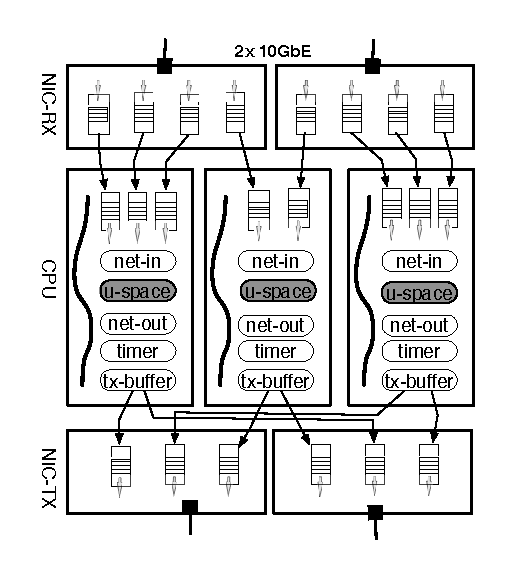
\includegraphics{figs/queues-cores.eps}

\vspace*{-0.25in}\caption{Example of IX scaling across two NICs interfaces, 8 NIC RX queues, and 3 CPU hardware threads.} 

\label{fig:queues-cores}
\end{figure}




\myparagraph{Flow consistent, coherence-free processing:} We use multi-queue
NICs with RSS support to provide flow-consistent hashing of incoming
traffic to distinct hardware queues. Each queue is served by a single
hardware thread all the way to the application layer, eliminating the
need for synchronization and cache coherence traffic between
cores. Similarly, memory management is organized in distinct pools for
each hardware thread. The absence of a socket layer eliminates the
issue of the shared file descriptor namespace in multithreaded applications~\cite{DBLP:conf/sosp/ClementsKZMK13}. Hence,
our design scales well with the increasing number of cores in modern
servers. Our approach does not restrict the memory model for
applications. Application logic can take advantage of coherent, shared
memory to exchange information and synchronize between cores. 


% \christos{seems like an implementation detail to me}
%The approach extends to link-aggregation bonds to scale to multiple links.


\myparagraph{Buffering at the NIC edge:} The consequence of adaptive
batching is the buildup of queues at the NIC edge before the packets
are processed by the dataplane.  Because of the dataplane's design,
congestion occurs only at the NIC edge.  In effect, the NIC edge acts
like the last-hop buffer in the network.  This has an additional
benefit in terms of flow control, as the networking stack sends
acknowledgments to peers only as fast as the application can process
them.  Congestion in the NIC edge therefore leads to shrinking windows
in peers, and flow control.


Like switches and routers, the NIC edge can
monitor queue depths to detect congestion, signal the control plane to
allocate additional resources (more hardware threads, increase clock
frequency) for the dataplane, notify explicitly flow sources of
congestion (e.g., via ECN~\cite{ramakrishnan2001addition}), and finally make
policy decisions when it is necessary to manage congestion (e.g., via RED~\cite{DBLP:journals/ton/FloydJ93}).




\section{\ix Implementation}
\label{sec:impl}

\begin{table*}[t]
\centering
\begin{small}
\begin{tabular}{|c|c|c|}
\hline
\multicolumn{3}{|c|}{Event Conditions (each has a cookie, not shown)} \\
\hline
Condition &           Parameters  &                             Description\\
\hline
Knock  &               cookie,src\_IP, src\_port &                        A remote host is attempting to open a connection \\
Connected &            cookie,outcome  &                                  A locally initiated flow has finished connecting\\
Recv &                 cookie, mbuf\_ptr, mbuf\_len &                  A message buffer has been received\\
Sent &                 cookie, bytes\_sent, window\_size &          Packet transmission has completed and/or the window size has changed \\
Dead &                cookie, reason &                                    The flow has been closed or an error has occurred \\
\hline
\hline
\multicolumn{3}{|c|}{Batched System Calls (partial list)} \\
\hline
connect &            cookie, dst\_IP, dst\_port &            Open a connection\\
accept &               handle, cookie &                          Accept a connection\\
sendv &               handle, scatter\_gather\_array &      Transmits an array of addresses and lengths\\
recv\_done &          handle, bytes\_acked &                Advances the receive window and frees memory buffers\\
close &                 handle &                                      Closes a connection\\
\hline
\end{tabular}
\caption{\ix event conditions and batch system calls}
\label{tbl:api}
\end{small}
\end{table*}



We now describe the \ix prototype.  The current implementation uses
the VT-x features available on all x86-64
servers~\cite{DBLP:journals/computer/UhligNRSMABKLS05}. However, it can
be ported to any architecture with virtualization support, such as ARM
and Power.

% We start
% with an overview of the \ix kernel (\S\ref{sec:impl:kernel}), describe
% the environment surrounding \ix (\S\ref{sec:impl:env}), and how \ix is
% implemented as a coherency-free kernel (\S\ref{sec:impl:cohfree}).


%the benefits of having \ix run as a guest
%operating system (\S\ref{sec:impl:guest}), its native API at the
%kernel/user boundary (\S\ref{sec:impl:api}), the implementation of the
%networking stack (\S\ref{sec:impl:stack}), the implications on
%congestion management and flow control (\S\ref{sec:impl:net}), the
%benefits and consequences of coherence-free execution
%(\S\ref{sec:impl:cohfree}), and finally our approach to compatibility
%(\S\ref{sec:impl:libix}).

\subsection{Overview}
\label{sec:impl:overview}

Fig.~\ref{fig:cp-dp} presents the \ix architecture, including the
control plane, a number of dataplanes, and applications. The hardware
environment includes one or more multi-queue NICs with RSS support and
a multi-core server.

The \ix control plane consists of the full Linux kernel and
\texttt{IXCP}, a user-level program. The Linux kernel initializes PCIe
devices, such as the NICs, and provides the basic mechanisms for
resource allocation to the dataplanes, including cores, memory, and
network queues. Equally important, Linux provides
system calls and services that are necessary for compatibility with a wide
range of applications, such as file system and signal
support. \texttt{IXCP} monitors resource usage and dataplane
performance and implements resource allocation policies. The
development of efficient allocation policies involves understanding
difficult tradeoffs between dataplane performance, energy
proportionality, and resource sharing between co-located applications
as their load varies over time. \george{is any christos' paper relevant for citation here?} We leave the design of such policies
to future work and focus this paper on the \ix dataplane architecture.

We run the Linux kernel in VMX root ring 0, the mode typically used to
run hypervisors in virtualized
systems~\cite{DBLP:journals/computer/UhligNRSMABKLS05}. We use the
Dune system within Linux to enable dataplanes to run as library-based
OSes in the VMX non-root ring 0, the mode typically used to run guest
kernels in virtualized systems~\cite{belay2012dune}. Finally, applications run
in VMX non-root ring 3. This approach provides dataplanes with direct
access to hardware features, such as page tables and exceptions, and provides full
protection between the control plane, dataplanes, and untrusted user
code. %\christos{should we explicitly say that most web-scale apps are
%  deployed without VMs so taking over VMX is not a problem?}\edb{not needed}

% \myparagraph{Separation and protection of control and data plane:}
% Each \ix instance and its applications runs as a distinct Dune process
% while control plane functions, including the control and monitoring of
% dataplane, is performed by scripts and daemons of the host
% environments.  This provides protection between control and
% dataplanes. Within each dataplane, \ix further protects itself from
% the untrusted application through virtual memory and by running it at
% userlevel.

% Section Move to the discussion session or future work
% \myparagraph{Elasticity policies:} In contrast to the mechanisms,
% which are generic, different policies can be envisioned to meet
% different use cases and optimization functions.  If neither energy
% proportionality or server consolidation is of any concern, the control
% plane can obviously launch a single dataplane instance configured with
% the maximal available physical resources.  In more realistic
% scenarios, the dataplane is ``right-sized'' to meet its service-level
% agreements with minimal resource allocations.  The control plane can
% further dynamically add or revoke CPUs from a dataplane instances,
% e.g., when the dataplane signals some sustained congestion or
% violation of its service-level agreements, or conversely when the
% allocated CPU resources are underutilized.


Each \ix dataplane supports a single, multithreaded POSIX
application. For instance, Fig.~\ref{fig:cp-dp} shows one dataplane
for a multi-threaded \texttt{memcached} server and another dataplane
for a multi-threaded \texttt{nginx} server. The control plane allocates
resources to each dataplane in a coarse-grain manner. Core allocation
is controlled through real-time priorities and \texttt{cpusets};
memory is allocated in large pages of 2MB in size; each NIC hardware queue is
assigned to a single dataplane. This approach avoids the overheads and
unpredictability of fine-grain time multiplexing of resources between
demanding applications~\cite{Leverich:RHSU:2014}.

The \ix dataplane operates as a single address-space OS and supports
two thread types within the shared, user-level address space: (i)
\emph{elastic threads} which interact with the \ix dataplane to
initiate and consume network I/O and (ii) \emph{background threads}.
Both elastic and background threads can issue arbitrary POSIX system
calls that are \adam{new:} intermediated and validated for security
by the dataplane before being being forwarded
by the Linux kernel.  Elastic threads are expected to \emph{not} issue
blocking calls because of the adverse impact on network behavior and
performance. Similarly, each elastic thread makes exclusive use of a
core or hyperthread allocated to the dataplane in order to achieve
high performance with predictable latency. In contrast, multiple
background threads may timeshare an allocated hyperthread. For example, if an
an application were allocated four hyperthreads, it could
use all of them as elastic threads to serve external requests or it could
temporarily transition to three elastic threads and use one background thread
to execute tasks such as garbage collection. When the control plane
revokes or allocates an additional hyperthread using a protocol
similar to the one used in Exokernel~\cite{DBLP:conf/sosp/EnglerKO95},
the dataplane must adjust the number of elastic threads it uses.

% We extended the Dune sandboxing mechanisms to support the initial load
% of multi-threaded applications into the userlevel address space, to
% launch both elastic and background threads.

\subsection{Dataplane API and Operation}
\label{sec:impl:kernel}

Elastic threads interact with the \ix dataplane through three
asynchronous, non-blocking mechanisms summarized in
Table~\ref{tbl:api}: they can issue \emph{batched systems calls} to
the dataplane; they consume \emph{event conditions} generated by the
dataplane; and they have direct, but safe, access to message buffers
(\emph{mbuf}) containing incoming networking payload. The latter is
quite different from traditional POSIX I/O and allows for
zero-copy access to incoming network traffic.  The application can
hold on to these message buffers until it asks the dataplane to release them via a batched
system call.  \ix also differs in directly exposing flow control
conditions to the application. The \texttt{sendv} system call does
not return the number of bytes buffered. \adam{new:} Instead,
it indicates the number of bytes that were accepted and immediately sent by
the TCP stack, as constrained by correct TCP sliding window operation. Then,
when the bytes are acknowledged by the receiver, a \texttt{sent} event
condition informs the application that it is possible to send more data. Thus send
window sizing policy is determined entirely by the application.
By constrast, todays OSes buffer send data (beyond raw TCP constraints) and
apply flow control policy inside the kernel ~\cite{dynamicwindow}.

\adam{not sure where to put this, but handles are kernel identifiers. Cookie's are
user-level identifiers that are associated, by the application, with kernel
handles. As a result, the user never has to look up an array or hash table to
find its flow metadata. It just casts the cookie as a pointer and references
it directly. This turns out to be a cool optimization because it alleviates
the file descriptor number is lowest available requirement, which is not communative.
The reason for this requirement appears to be to allow user apps to easily make tables
of meta-data pointers for each file descriptor.}

In addition to the low-level native \ix API in Table~\ref{tbl:api}, we also
built a user-level library that provides a compatible programming
model for legacy applications and significantly simplifies the
development of new applications. \adam{new:} Our library
provides a functionally compatible interface to \texttt{libevent} and non-blocking
POSIX socket operations. It also includes new
interfaces for zero copy read and write operations that are more efficient,
at the expense of requiring larger changes to existing applications. However, We
are still missing certain features in our prototype implementation, such as
support for timer events and high-level buffered I/O utilities.

\begin{figure*}
%\hspace*{-0.25in}\centering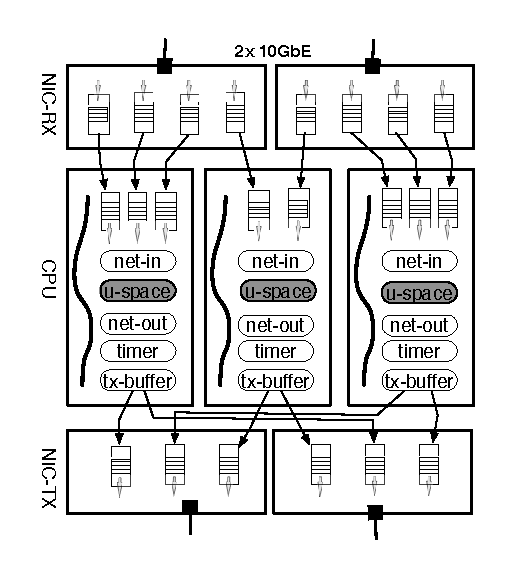
\includegraphics{figs/queues-cores.eps}
%\centering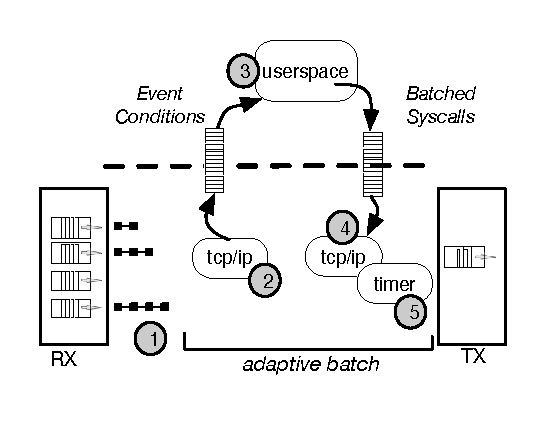
\includegraphics{figs/pipeline}
\subfloat[Switches and NICs split traffic into flow-consistent groups]{
\label{fig:rss}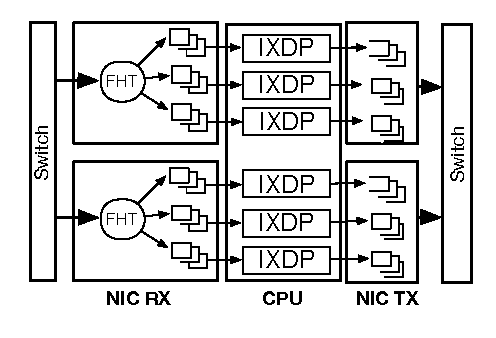
\includegraphics{figs/rss}}
\hspace*{1em}
\subfloat[Interleaving of protocol processing and application execution]{
\label{fig:dataplane}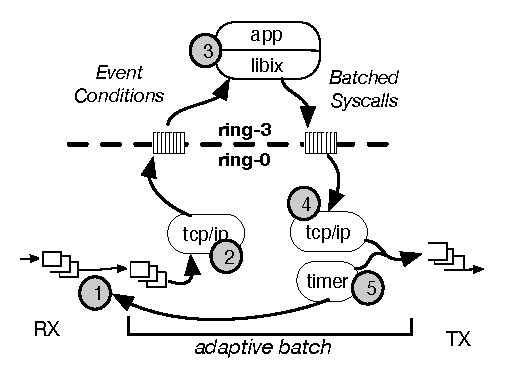
\includegraphics{figs/pipeline-2}}

\caption{The IX dataplane}
\label{fig:queues-cores}
\end{figure*}


\begin{comment}
\dm{Make clear how this corresponds to
    figure 1---i.e., that the dotted line separates ring 3 from VMX
    non-root ring0.  Also, this diagram makes it look like there are
    big queues, contradicting the process to completion idea.  Maybe
    use a different abstraction for queues vs.\ batches (which I
    assume is what is being depicted across the dotted line).  Finally
    the diagram should close the loop in some way.  I.e., do you go
    straight from 5 (really 6 should be depicted0 back to 1, or do you
    invoke a scheduler or check if you need to relinquish the core at
    that point?}}
\end{comment}

 

Fig.~\ref{fig:queues-cores} illustrates the run-to-completion
operation of elastic threads in the \ix dataplane. Each elastic thread
is associated with a specific set of receive queues from one or more
NICs. Each NIC uses RSS to implement flow-consistent hashing and
distribute incoming packets to queues. The queues are mapped in the
server's main memory and the NIC is given a set of buffer descriptors
that allow it to transfer incoming packets to memory using DMA.  The
elastic thread (1) polls the receive queues it is responsible for and
potentially posts fresh buffer descriptors to the NIC for use with
future incoming packets. The elastic thread (2) processes a bounded
number of packets through the TCP/IP networking stack, thereby
generating event conditions. Next, the elastic thread (3) passes
control to the user-space applications, which consumes all event
conditions. Assuming that the incoming packets include remote
requests, the application processes these requests and responds with a
batch of system calls. Upon return of control from user-space, the
elastic thread (4) processes all system calls, and in particular the
ones that direct outgoing TCP/IP traffic. It also (5) runs all kernel
timers in order to ensure compliant TCP behavior and (6) places
outgoing Ethernet frames in the NIC's descriptor rings for
transmission. Finally, it notifies the NIC to initiate a DMA transfer
for these frames by updating the transmit ring's tail register. 

The \ix dataplane consists of 37 KSLOC. We leveraged existing
codebases in its development: 43\% is derived from the DPDK variant of
the Intel NIC device driver~\cite{intel:dpdk}, 23\% from the lwIP TCP/IP
stack~\cite{dunkels2001design}, and 16\% from the Dune library.  All
three code bases are highly modified for \ix. The rest is
approximately 7 KSLOC of new code. We chose lwIP as a starting point
for TCP/IP processing because of its modularity and its maturity as a
compliant, feature-rich networking stack. It allows us to be
RFC-compliant for TCP, UDP, ARP, and ICMP. \adam{actually we implemented our own UDP, ARP, and ICMP, but not sure if this matters}
Since lwIP was optimized for memory efficiency in embedded environments, we had to
radically change its internal data structures for multi-core
scalability and fine-grain timer management. We did not yet optimize
the lwIP code for performance. Hence, there is room for improvement in
the results shown in \S\ref{sec:eval}. 


\subsection{Multi-core Scalability}
\label{sec:impl:cohfree}

The \ix dataplane is optimized for multi-core scalability as elastic
threads operate in a synchronization and coherence free manner in the
common case. This is a stronger requirement than lock-free
synchronization, which requires expensive atomic instructions even
when a single thread uses a particular lock in the common
case~\cite{DBLP:conf/sosp/DavidGT13}.  This was made possible 
through a set of conscious design and implementation tradeoffs. 

First, the \ix API is commutative. Events are processed independently
on each elastic thread. Handles identify flows but cannot be exchanged
between elastic threads. There is no file descriptor namespace.
According to the commutativity rule, system call implementations can
only be coherence-free if the API itself is
commutative~\cite{DBLP:conf/sosp/ClementsKZMK13}.

Second, the API implementation is carefully optimized.  Each elastic
thread manages its own memory pools, hardware queues, event condition
queue, and batched system call queue. No synchronization is required
to access any of them. The implementation of event conditions and
batched system calls benefits directly from the explicit, cooperative
control flow transfers between \ix and the application by the elastic
thread.  Since there is no concurrent execution by producer and
consumer, event conditions and batched system calls are implemented
without relying on lock-free synchronization primitives based
on atomics.

Third, the use of flow-consistent hashing at the NICs ensures that
each elastic thread operates on a disjoint subset of incoming TCP
flows. Hence, no synchronization or coherence occurs during the
processing of incoming requests for a server application. For client
applications with outbound connections, we need to ensure that the
reply is assigned to the same elastic thread that made the
request. Since we cannot reverse the Toeplitz hash used by RSS, we
simply probe the ephemeral port range to find a port number that
would lead to the desired behavior. Note that this implies that two
elastic threads in a client cannot share a flow to a server. % \edb{\sout{In
% \S\ref{sec:eval}, we show that \ix scales wells to hundreds of
% thousands of outgoing connections.}}
 
% ephemeral source port no longer form namespaces, which allows an \ix
% client to support millions of outgoing connections.


% \ix selects the source ephemeral port based on
% the requesting elastic thread. Since the Toeplitz hash function cannot
% be reversed, \ix simply probes the ephemeral range and computes the
% Toepliz hash until a match is found.  


\ix does have a small number of shared structures, including some that
require synchronization on updates.  For example, the ARP table is
shared by all elastic threads and is protected by RCU
locks~\cite{mckenney1998read}, Hence, the common case reads are
coherency-free but the rare updates are not. \ix also requires
synchronization when the control plane reallocates resources between
dataplanes.  For instance, when a core is revoked from a dataplane,
the corresponding incoming queues must be assigned to another elastic
thread. Such events are rare because resource allocation happens in a
coarse-grain manner. Finally, the application code may include
inter-thread communication and synchronization. While using \ix does
not eliminate the need to develop scalable application code, it
ensures that there are no scaling bottlenecks in the system and
protocol processing code. 

\subsection{Cooperative Flow Control}
\label{sec:impl:coop}

\adam{rename this section ``Security Design/Model'' ?}

The \ix API and implementation leads to a cooperative flow control
model between application code and the network-processing stack.  But
unlike user-level stacks that also expose networking behavior to user
code, the \ix protection model makes few assumptions about application
behavior. A malicious or misbehaving application can only hurt
itself. It cannot corrupt the networking stack or affect other
applications.

The \ix dataplane and the application collaboratively manage
memory. To enable zero-copy operation, a buffer used for an incoming
packet is passed read-only to the application, enabling zero-copy
operation. Applications that hold on to message buffers for extensive
periods of time must bound their use of this shared resource.  In the
transmit direction, zero-copy operation implies that the application
must maintain outgoing data immutable until the reception is
acknowledged by the peer. % \edb{\sout{If there is recepient is not
    % operating fast enough or there is network congestion, the sender
    % will soon experience memory pressure as well.}}

Since elastic threads in \ix execute both the network stack and
application code, a long running application can block further network
processing for a set of queues. This behavior affects no other
applications or dataplanes in anyway. We use a timeout interrupt to
detect elastic threads that spend excessive time in user mode (e.g.,
beyond 10ms). We mark such applications as non-responsive and notify
the control plane. %\edb{\sout{to potentially take resource allocation actions.}}

Note that all application code in \ix runs in user-mode, while the
dataplane code is in protected ring 0. Applications cannot access
kernel memory, except for read-only message buffers, or network
hardware.  No sequence of batched system calls or other user-level
actions can be used to violate correct adherence to TCP and other
network specifications.  Furthermore, the dataplane can be used to
enforce network security policies (e.g., iptables or Amazon Security
Groups~\cite{url:amazon-sg}) or to implement the network virtualization functions typically
done in a hypervisor~\cite{nsdi:nsx}. Our security model is as strong
as conventional network stacks in commodity OSes and is missing from all
the recently proposed user-level networking stacks.

\adam{new:} Our prototype implementation does not yet support IOMMUs, and as a result,
a dataplane could potentially corrupt control plane memory through stray DMA operations.
However, unlike user-level network stacks we do not strickly require IOMMU support, as untrusted
application code is never is given direct access to NIC DMA engies. Rather, adding
IOMMU support would improve security by creating a layer of defense in depth between
dataplanes and control planes, possibly at the expensive of some performance
overhead~\cite{iommu_overhead}.




\section{Evaluation}
\label{sec:eval}

\subsection{Experimental setup}
\label{sec:eval:setup}


\todo Compare apples-to-apples with Megapipe, and mTCP in terms of microbenchmarks.

\todo Baseline comparison of state-of-the art systems include:  Linux (some recent version, with SO\_REUSEPORT); Megapipe (if possible), mTCP (if possible). 

\todo Microbenchmark: short TCP transactions (echo server, as defined in megapipe).   Goal is to beat mTCP (and therefore all others) hands down.

\todo Benchmark: memcached - compare with FB results (?)

\todo Benchmark: lightttpd -- used by Affinity-Accept and mTCP.  

\todo ngnx: an actually used webserver.



\section{Discussion}
\label{sec:disc}


\myparagraph{What makes \ix fast:} The results in \S\ref{sec:eval}
show that a networking stack can be implemented in a protected OS
kernel and still deliver wire-rate performance for most benchmarks.
The tight coupling of the dataplane architecture, using only a minimal
amount of batching to amortize transition costs, causes application
logic to be scheduled at the right time, which is essential for
latency-sensitive workloads.  Therefore, the benefits of \ix go beyond
just minimizing kernel overheads. The lack of intermediate buffers
allows for efficient, application-specific implementations of I/O
abstractions such the \texttt{libix} event library. The zero-copy
approach helps even when the user-level libraries add a level of
copying, as it is the case for the \texttt{libevent} compatible
interfaces in \texttt{libix}.  The extra copy occurs much closer to
the actual use, thereby increasing cache locality.  Finally, we
carefully tuned \ix for multi-core scalability, eliminating constructs
that introduce synchronization or coherence traffic.



\myparagraph{Subtleties of adaptive batching:} Batching is commonly
understood to trade off higher latency at low loads for better
throughput at high loads.  \ix uses adaptive, bounded batching to
actually improve on both metrics.  Fig.~\ref{fig:batch-mutilate}
compares the latency vs. throughput on the \texttt{USR}
\texttt{memcached} workload of Fig.~\ref{fig:mutilate} for different
upper bounds $B$ to the batch size.  At low load, $B$ does not impact
tail latency, as adaptive batching does not delay processing of
pending packets.  At higher load, larger values of $B$ improve
throughput, by 23\% between $B=1$ to $B=16$.  For this workload, $B
\ge 16$ maximizes throughput.


\begin{comment}
\myparagraph{Subtleties of adaptive batching:} 
Batching is commonly understood to trade off higher latency at low loads
for better throughput at high loads.  Our use of adaptive, bounded
batching actually improves on both metrics. In exploring the impact of
the batch size bound --- which impacts behavior when the workload is
CPU-bound --- we first confirmed the intuition that larger batch
sizes improve throughput, but only to a point. Fig.~\ref{fig:batch}
compares the throughput of the CPU-bound benchmark used in
Fig.~\ref{fig:short10:roundtrips}.  The experiment shows that batches
as low as $B=32$ can deliver maximal throughput for this
workload. (All experiments in \S\ref{sec:eval} were conducted with a
maximal batch size of $B=64$ packets per iteration.)  Because the
algorithm is adaptive, $B$ does not impact latency when the dataplane
is not saturated; we confirmed
this experimentally at the 99th percentile latency for
\texttt{memcache}.
\end{comment}


%\begin{figure}
\begin{centering}
\includegraphics{figs/batch.eps}
\caption{Throughout of a CPU-bound microbenchmark for different values of batch size.}
\label{fig:batch}
\end{centering}
\end{figure}


\begin{figure}
\begin{centering}
\includegraphics{figs/batch-mutilate.eps}
\caption{99th percentile latency as a function of throughput for \texttt{USR} workload from Fig.~\ref{fig:mutilate}, for different values of the batch bound $B$.}
\label{fig:batch-mutilate}
\end{centering}
\end{figure}



While tuning \ix performance, we ran into an unexpected hardware limitation
that was triggered at high packet rates with small average batch sizes 
(i.e. before the dataplane was saturated): 
the high rate of PCIe writes required to post fresh
descriptors at every iteration led to performance degradation as we
scaled the number of cores.  To avoid this bottleneck, we
simply coalesced PCIe writes on the receive path so that we
replenished at least 32 descriptor entries at a time.  Luckily, we did
not have to coalesce PCIe writes on the transmit path, as that would
have impacted latency.


\begin{comment}
  \myparagraph{Using interrupts as a fallback:} Some applications
  service requests that require extended intervals of compute time. We
  intend for these requests to be delegated to from elastic threads to
  background threads in order to ensure that elastic threads remain
  responsive.  However, \ix can also be modified to better tolerate
  unanticipated delays during application processing in elastic
  threads.  One option would be to use interrupts as a fallback
  mode. On the receive side, the NIC would fire an interrupt whenever
  the recieve descriptor ring is almost full. The dataplane could then
  move packets from the receive ring to a software structure, averting
  buffer underrun. On the transmit side, NIC would fire an interrupt
  whenever the transmit ring becomes empty so that it can be
  refilled. Such an interrupt would only need to be armed when there
  is additional transmit data pending. A desirable property of this
  approach is that neither interrupt would be triggered as long as
  elastic threads are sufficiently responsive, but if an elastic
  thread misbehaves, the \ix dataplane would be able to regain control
  and catch up on network processing.
\end{comment}


\myparagraph{Limitations of current prototype:} The current \ix
implementation does not yet exploit IOMMUs or VT-d. Instead, it maps
descriptor rings directly into \ix memory, using the Linux pagemap
interface to determine physical addresses.  Although this choice puts
some level of trust into the \ix dataplane, application code remains
securely isolated. In the future we plan on using IOMMU support to
further isolate \ix dataplanes. We anticipate overhead will be low
because of our use of large pages.  Also, the \ix prototype currently
does not take advantage of the NIC's SR-IOV capabilities, but instead
allocates entire physical devices to dataplanes.

We also plan to add support for interrupts to the \ix dataplanes. The
\ix execution model assumes some cooperation from application code
running in elastic threads.  Specifically, applications should handle
events in a quick, non-blocking manner; operations with extended
execution times are expected to be delegated to background threads
rather than execute within the context of elastic threads.  The \ix
dataplane is designed around polling, with the provision that
interrupts can be configured as a fallback optimization to refresh
receive descriptor rings when they are nearly full and to refill
transmit descriptor rings when they are empty (steps (1) and (6) in
Fig~\ref{fig:dataplane}). Occasional timer interrupts are also
required to ensure full TCP compliance in the event an elastic thread
blocks for an extended period.

\myparagraph{Future work:} This paper focused primarily on the \ix
dataplane architecture. \ix is designed and implemented to support the
dynamic addition and removal of elastic threads in order to achieve
energy proportional and resource efficient computing. So far we have
tested only static configurations. In future work, we will explore
control plane issues, including a dynamic runtime that rebalances
network flows between available elastic threads in a manner that
maintains both throughput and latency constraints.

We will also explore the synergies between \ix and networking
protocols designed to support microsecond-level latencies and the
reduced buffering characteristics of \ix deployments, such as
DCTCP~\cite{DBLP:conf/sigcomm/AlizadehGMPPPSS10} and
ECN~\cite{ramakrishnan2001addition}. Note that the \ix dataplane is
not specific to TCP/IP. The same design principles can benefit
alternative, potentially application specific, network protocols, as
well as high-performance protocols for non-volatile memory
access. Finally, we will investigate library support for alternative
APIs on top of our low-level interface, such as
MegaPipe~\cite{DBLP:conf/osdi/HanMCR12}, cooperative
threading~\cite{DBLP:conf/sosp/BehrenCZNB03}, and rule-based
models~\cite{DBLP:conf/hotos/StutsmanO13}.

%The current prototype
%supports any stateless offload NIC with multiple queues and RSS
%support.  \ix load balances RSS flow groups onto queues, but we plan
%to explore using Intel's Flow Director~\cite{intel:82599} for outbound
%connections rather than reversing the Toeplitz hash.



\section{Related Work}
\label{sec:related}

We organize the discussion topically, while avoiding redundancy with
the commentary already exposed in \S\ref{sec:motivation:current}.


\myparagraph{Virtualization hardware:} Hardware support for
virtualization naturally separates control and execution functions,
e.g., to build type-2 hypervisors
~\cite{DBLP:journals/tocs/BugnionDRSW12,misc/kivity07kvm}, run virtual
appliances~\cite{DBLP:conf/lisa/SapuntzakisBCZCLR03}, or processes
with access to privileged instructions~\cite{belay2012dune}.
Arrakis~\cite{peter2013arrakis,arrakisTR13} uses virtualization
hardware, the Barrelfish
multikernel~\cite{DBLP:conf/sosp/BaumannBDHIPRSS09} for control, and
its own networking stack, to separate the dataplane from the control
plane. \ix is a dataplane operating system that uses Linux for
control, Dune for isolation, a mature networking stack for protocol
processing.


\myparagraph{Library operating systems:}
Exokernels proposed to implement system abstractions via library
operating systems linked in with
applications~\cite{DBLP:conf/sosp/EnglerKO95}, extending the
end-to-end principle~\cite{DBLP:journals/tocs/SaltzerRC84} to the
management of system resources.  Library operating systems typically
run as virtual machines ~\cite{DBLP:journals/tocs/BugnionDGR97},
e.g. to deploy cloud services
~\cite{DBLP:conf/asplos/MadhavapeddyMRSSGSHC13}. The \ix kernel limits
itself to the implementation of protocol stack, allowing applications
to implement their own resource management policies, e.g. via the
\texttt{libevent} compatibility layer.


\myparagraph{User-level networking stacks:} User-level network
stacks~\cite{jeong2014mtcp, marinos2013network, openonload} can
outperform kernel-based implementations through specialization and
elimination of redundant layers and abstractions, but trade-off
performance for a weaker security model.  The \ix dataplane
demonstrates that a specialized networking stack can offer performance
and cooperate with applications without having to weaken security and
isolation properties.
 

\myparagraph{Hardware and protocol specialization:} 
Applications can use a connection-less UDP-based protocol for
scalability~\cite{nishtala2013scaling}.  Latency-sensitive datacenter
applications can use specialized Infiniband adapters to expose RDMA
with $1-3$\microsecond latencies to
applications~\cite{DBLP:conf/sosp/OngaroRSOR11,Jose:2011:MDH,mitchell:rdma,dragojevic14farm}.
Specialized FGPAs can replace conventional servers for important
applications such as
memcached~\cite{DBLP:conf/fpga/ChalamalasettiLWARM13}.  \ix is
designed to allow TCP/IP to scale with architectural trends by
elminating kernel bottlenecks.


\myparagraph{Asynchronous and zero-copy interactions:} 
Systems with asynchronous, batched, or exception-less system calls
substantially reduce the overheads associated with frequent kernel
transitions and context switches~\cite{
  soares2010flexsc,han2012megapipe,rizzo2012netmap,jeong2014mtcp}.
Zero-copy reduce data movement overheads and simplifies resource
management~\cite{DBLP:journals/tocs/PaiDZ00}.  \ix's use of adaptive,
bounded batching is suitable for both low-latency and high-message
rate, and its safe, cooperative memory management model enables
zero-copy at the application level.




\section{Conclusion}

We have presented \ix, a dataplane operating system for event-driven,
web-scale applications.  Our architecture leverages hardware
virtualization to separate the control plane, the \ix dataplane
instances, and the event-driven applications running on top of it.
\ix optimizes for both bandwidth and latency by processing bounded
batches of packets to completion and by eliminating coherence traffic
and synchronization on multi-core systems. We show that \ix
outperforms Linux 3.11 by an order of magnitude and mTCP by up to 2.5
in terms of throughput. It also outperforms Linux and mTCP in terms of
latency by 3x and 13.7x respectively. \ix can support efficiently a
hundred thousand connections. Finally, we show that porting
\texttt{memcached} to \ix removes kernel bottlenecks and improves
throughput by up to 2.7x.


% The system is designed to ensure high packet rates, to offer
% micro-second latency response times to clients including in high
% occupancy situations, to scale to a large number of TCP connections,
% and to allow for a coarse-grain, yet elastic allocation of hardware
% resources.


\section*{Acknowledgements}

\begin{itemize}
\item Carlos Perez (EPFL) last minute IT setup
\item Detailed comments: Jacob Leverich, Jim Larus
\item High-level comments: Katerina Argyraki
\end{itemize}




\bibliography{../common/dblp,../common/gscholar,../common/misc}
\bibliographystyle{abbrv} 

\ifcomments



\subsection{Latex sizes}

XXX REMOVE ME XXX

\begin{itemize}

\item colummwidth: \the\columnwidth
\item textwidth:  \the\textwidth
\item parskip: \the\parskip
\item abovecaption: \the\abovecaptionskip
\item belowcaption: \the\belowcaptionskip


\end{itemize}

\subsection{Misc. to cite}

Stuff to cite (that is not otherwise cited) ... that we should either incorporate or drop:



\begin{enumerate}

\oldcite{Corey OS}{DBLP:conf/osdi/Boyd-WickizerCCMKMPSWDZZ08}
\oldcite{Thekah -- early User-level networking}{DBLP:conf/sigcomm/ThekkathNML93}

\oldcite{Libra JVM}{DBLP:conf/vee/AmmonsABSGKKRHW07}
\oldcite{Scheduler activations}{DBLP:journals/tocs/AndersonBLL92}
%\oldcite{Atikoglu - Workload analysis fo large-scale key-value store}{Atikoglu:2012:WAL}
\oldcite{Basu - Efficient virutal memory for big memory servers}{DBLP:conf/isca/BasuGCHS13}
\oldcite{RadixVM}{DBLP:conf/eurosys/ClementsKZ13}
%\oldcite{Waldspurger - CPU balloning}{DBLP:conf/osdi/Waldspurger02}
%\oldcite{Drepper - cost of virtualization}{DBLP:journals/queue/Drepper08}
\oldcite{Thialfi}{DBLP:conf/sosp/AdyaCMP11}
%\oldcite{Cavium Octeon}{cavium-octeon}
\oldcite{Fan 2013 Mem Cache 3}{fan2013memc3}
%\oldcite{Case against userlevel networking}{magoutis2004case}


\ana{Could cite Harchol-Balter, Schroeder, Bansal, and Agrawal. Size-based Scheduling to Improve Web Perfomrance.}


\ana{Should cite Mogul and Ramakrishnan. Eliminating Receive Livelock in an Interrupt-Driven Kernel.}


\ana{From OSDI program committee, might consider citing: Emin Gun Sirer and Nick Feadmster.}

\end{enumerate}

\subsection{Dangling from related work}


\paragraph{Adaptive, batched run to completion}

\todo TODO

\paragraph{Coherence-free, flow-consistent processing}

\todo Affinity Accept, mTCP, ...



\paragraph{API design.}


\paragraph{Hardware specialization - Dataplanes.}

\paragraph{Operating system architecture.}

\paragraph{Domain-specific and library operating systems.}




%%%
%%%  use the ping-pong test to measure the half rountrip latency @ 64B
%%% 

\begin{table}[b]
\vspace{-1em}
\begin{center}
\begin{small}
\begin{tabular}{|l|c|c|c|}
\hline
Workload &  Avg lat. & 99\% lat. & Size\@5Gpbs\\
\hline
Linux(base) & 48\microsecond & 0\microsecond & 384KB\\
Linux(opt)    & 0\microsecond &  0\microsecond & XXX \\
mTCP    & 0\microsecond &  0\microsecond & XXX \\
\ix          & 32\microsecond &  39\microsecond & XXX\\
\ix-\ix                  & 17\microsecond &  0\microsecond & XXX\\
\hline
\end{tabular}
\caption{Netpipe half-roundtrip latency (s=64B)}
\vspace*{-2em}
\label{tbl:pingpong}
\end{small}
\end{center}
\end{table}



\fi

%
\section{Internal Notes}

\subsection{Christos notes}

From email on 14-10-09. There are many issues that can complicate the CP. Here is unordered list:

\begin{itemize}

\item Measuring or inferring latency reliably, especially in the presence of many different request types. 
\item  limited queues. 128 queues or flow groups may not be enough. My students interning at Google were already using servers with 72 hardware threads. That’s were the flow director may be useful. 

\item  interactions with TurboBoost  (initially we should keep it off)
\item  it would be great of CP balancing allows us to use the 2nd socket efficiently (initially we should start with a single socket)
\item rate limiting: what if I want to deploy memcache so that it takes at most N cores. When we use all of them and we get too much queuing, how do we rate limit/drop requests to maintain some SLA? 

\end{itemize}


The other important thing to do is to enumerate test scenarios. Here is my list:
\begin{itemize}

\item energy proportionality: showily scale from 0\% to 100\% load for
  memcached and show that CP does the best possible thing for SLA and
  EP

\item energy proportionality: do we few tests of rapid change between load to characterize transition time issues
\item  sharing: slowly scale from from 0\% to 100\% the load for memcached and show that all other cores can be kept busy with a non interfering benchmark (while 1). The metric is the progress rate of the other benchmark

\item sharing: rapid change to load to characterize reaction time

\item interference: slowly scale from from 0\% to 100\% the load for memcached and show that all other cores can be kept busy with a interfering benchmarks. Initially run the same interfering benchmark on all other cores. The metric is the memcache SLA and the progress rate of the other benchmark. 

\item interference: rapid change to memcached load. 
\item interference; rapid change to the ether benchmark (e.g., from while 1 to a cache interfering one). 
\end{itemize}


A great tool for NUMA isolation: 
http://www.open-mpi.org/projects/hwloc/
The lstopo and hwloc-bind tools seem VERY very useful for what we are doing. Take a look. 


\subsection{Ed notes}

Guri Sohi's varona\cite{DBLP:conf/pldi/SridharanGS14} efficiently adapts to parallelism.


\subsection{Citations with aliases:}


\begin{itemize}
\item Dune: \cite{dune}
\item megapipe: \cite{megapipe}
\item Sandstorm: \cite{sandstorm}
\item Click: \cite{click}
\item Routebricks: \cite{routebricks}
\item Aikoglu \cite{Atikoglu:2012:WAL}
\item Tinyosnet: \cite{tinyosnet}
\item Quasar: \cite{quasar}
\item mtcp: \cite{mtcp}
\item Arrakis: \cite{arrakis-osdi}
\end{itemize}

 % really old stuff



\end{document}

